\section{Combining Scope Graphs with Types}
\sectionlabel{by-example}

In this section we describe our approach to type-dependent name resolution using
examples in a small model language. We show how scope graphs are used to model
name binding, combine scope graphs with type constraints to model type
resolution, and discuss extension of the two models to handle type-dependent
name resolution.

\subsection{Example Language}

We illustrate the ideas using LMR (Language with Modules and Records), which 
extends the LM (Language with Modules) of \cite{NeronTVW-ESOP-2015}.
The language does not aspire to be a real programming language, but is designed
to represent typical and challenging name and type resolution idioms.
The grammar of LMR is defined in \Figure{lmr:grammar}.
The basic features that LMR inherits from LM are:
\begin{itemize}
  \item Modules and imports: modules can be nested and can import other modules.
  \item Various flavours of variable binding constructs: variable
  definitions (\cod{def}), first-class functions (\cod{fun}), and three flavours
  of let bindings.
  \item Declarations (modules, definitions, records) in the same module
  (scope) are mutually recursive.
  \item Qualified names allow access to the declaration in a module without
  import.
\end{itemize}

\noindent
LMR extends LM with the following features:

\begin{itemize}
  \item LMR is statically typed: function arguments require explicit type
  annotations, but bindings of variables may be left for type inference to
  resolve.
  \item Declaration of nominal record types with inheritance and a corresponding
  subtyping relation on record types.
  \item Construction of (immutable) records with \cod{new} using references to fields for
  initialization.
  \item Access to the fields of a record value using dot notation \cod{e.f}.
  \item Implicit access to record fields using a Pascal-like \cod{with}
  construct.
\end{itemize}

\noindent In the rest of this section we study name and type resolution for a
selection of LMR constructs that explain the ideas of type-dependent name
resolution using examples. Subsequent sections formalize these ideas.
\begin{figure}[t]
\begin{boxedminipage}{\hsize}
\begin{grammar}
\sdnn{prog}{$\ks{\w{decl}}$}
\\
\sdnn{decl}{\kw{module}\ \w{Id}\ \sep{\{} \ks{\w{decl}} \sep{\}}}
\altf{\kw{import}\ \w{Qid}}
\altf{\kw{def}\ \w{bind}}
\altnn{\kw{record}\ \w{Id}\ \opt{\w{sup}}\ \sep{\{} \ks{\w{fdecl}} \sep{\}}}
\\
\sdnn{sup}{\kw{extends}\ \w{Qid}}
\\
\sdnn{fdecl}{\w{id}\ \sep{:}\ \w{ty}}
\\
\sdnn{ty}{\kw{Int}}
\altf{\w{Qid}}
\altf{\w{ty}\ \sep{->}\ \w{ty}}
\\
\sdnn{exp}{\w{int}}
\altf{\kw{true}}
\altf{\kw{false}}
\altf{\w{qid}}
\altf{\w{exp} \oplus \w{exp}}
\altnn{\kw{if}\ \w{exp}\ \kw{then}\ \w{exp}\ \kw{else}\ \w{exp}}
\altnn{\kw{fun}\ \sep{(}\ \w{id}\ \sep{:}\ \w{ty}\ \sep{)}\ \sep{\{} \w{exp} \sep{\}}}
\altf{\w{exp}\ \w{exp}}
\altnn{\kw{let}\ \ks{\w{bind}}\ \kw{in}\ \w{exp}}
\altf{\kw{letpar}\ \ks{\w{bind}}\ \kw{in}\ \w{exp}}
\altnn{\kw{letrec}\ \ks{\w{tbind}}\ \kw{in}\ \w{exp}}
\altnn{\kw{new}\ \w{Qid}\ \sep{\{} \ks{\w{fbind}} \sep{\}}}
\altf{\kw{with}\ \w{exp}\ \kw{do}\ \w{exp}}
\altnn{\w{exp}\ \sep{.}\ \w{id}}
\\
\sdnn{Qid}{\w{Id}}
\altf{\w{Qid}\ \sep{.}\ \w{Id}}
\\
\sdnn{qid}{\w{id}}
\altf{\w{Qid}\ \sep{.}\ \w{id}}
\\
\sdnn{bind}{\w{id}\ \sep{=}\ \w{exp}}
\altf{\w{tbind}}
\\
\sdnn{tbind}{\w{id}\ \sep{:}\ \w{ty}\ \sep{=}\ \w{exp}}
\\
\sdnn{fbind}{\w{id}\ \sep{=}\ \w{exp}}
%\mc{id}{identifiers}
%\\
%\mc{int}{integer constants}
\end{grammar}
\end{boxedminipage}
  \caption{Syntax of LMR.}
  \figurelabel{lmr:grammar}
\end{figure}



\subsection{Declarations and References}

\newcommand{\ric}[2]{\ri{\cod{#1}}{#2}}
\newcommand{\dic}[2]{\di{\cod{#1}}{#2}}

We recall the concepts of the scope graph approach \cite{NeronTVW-ESOP-2015} and
extend it with type constraints.
Consider the example in \Figure{var-ref}, which shows an LMR program (top), and
the scope graph diagram and constraints (below) extracted from it.
Subscripts on identifiers represent AST positions. Thus, \cod{x$_1$} and
\cod{x$_3$} are different occurrences of the \emph{same} name~\cod{x}.

\paragraph{Scope Graph}

The key building block of a scope graph is the \emph{scope}, an abstraction of a
set of nodes in the AST that behave uniformly with respect to name binding.
In a scope graph diagram, scopes are represented by circles with numbers
representing their identity.
Scopes manage the visibility of \emph{declarations}. In a diagram, declarations
are represented by boxes with an \emph{incoming arrow} from a scope.
In the example program \cod{x$_1$} and \cod{y$_2$} are declarations. In
constraints we denote declarations using a {\sf D} superscript (e.g.
$\dic{x}{1}$).
\emph{References} are identifiers that refer to a declaration.
In diagrams, a reference is represented by means of a box with an arrow pointing
to its scope.
In the program \cod{x$_3$} and \cod{x$_4$} are references.
In constraints we denote references with an {\sf R} superscript (e.g.
$\ric{x}{3}$).
\emph{Name resolution} in a scope graph consists of finding a path in the scope
graph from a reference to a declaration. Since scope 1 contains a declaration
$\dic{x}{1}$ with the name \cod{x}, both references $\ric{x}{3}$ and
$\ric{x}{4}$ resolve to the declaration $\dic{x}{1}$, which we write $\ric{x}{3}
\resolve \dic{x}{1}$.


\begin{figure}[t]
  \twoboxes{.495\hsize}{.495\hsize}{%
\small
Scope graph\\

\begin{center}
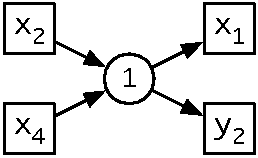
\includegraphics[scale=.5]{figures/examples/manual/01-variable-reference}
\end{center}
%
\begin{mconstraints}{Declarations}
\EqCType{\dic{x}{1}}{\tau_{1}} & 
\EqCType{\dic{y}{2}}{\tau_{2}} 
\end{mconstraints}
%
\begin{mconstraints}{Reference constraints}
\EqCResolve{\ric{x}{3}}{\delta_{1}} & 
\EqCType{\delta_{1}}{\intty{}}\\
\EqCResolve{\ric{x}{4}}{\delta_{2}} & 
\EqCType{\delta_{2}}{\tau_{4}}
\end{mconstraints}}{\small%
\begin{mconstraints}{Type constraints}
\EqCTeq{\tau_{1}}{\intty{}} \\ 
\EqCTeq{\boolty{}}{\boolty{}}\\
\EqCTeq{\intty{}}{\intty{}} \\ 
\EqCTeq{\tau_{3}}{\intty{}}\\
\EqCLub{\tau_{2}}{\tau_{3}}{\tau_{4}}
\end{mconstraints}%
\begin{mconstraints}{Solution}
\RCSubst{\delta_{1}}{\dic{x}{1}} & 
\RCSubst{\delta_{2}}{\dic{x}{1}}\\
\TCSubst{\tau_{1}}{\intty{}} & 
\TCSubst{\tau_{2}}{\intty{}}\\
\TCSubst{\tau_{3}}{\intty{}} & 
\TCSubst{\tau_{4}}{\intty{}}
\end{mconstraints}%
}

\begin{boxedminipage}[t]{\hsize}
  \lstinputlisting[language=LMR,basicstyle=\lstfigurestyle, frame=none]{figures/examples/01-variable-reference.lmr}
\end{boxedminipage}
\begin{boxedminipage}[t]{.495\hsize}
\usebox{\boxone}
\end{boxedminipage}
\hfill
\begin{boxedminipage}[t]{.495\hsize}
  \usebox{\boxtwo}%
  \vspace{\vdiff}
\end{boxedminipage}

\caption{Declarations and references in global scope with example program, scope graph, and constraints.}

  \figurelabel{var-ref}
\end{figure}

\paragraph{Type Constraints}

Scope graphs do not include explicit type information. 
However, by associating type information with identifier declarations, it is
easy to obtain the type of an identifier reference by first resolving the
reference to a declaration and then looking up the associated type information
by position in the AST.
However, that requires a language-dependent mechanism. 
In order to abstract from the language-specific representation of type
information in the AST, we generate constraints in a language-independent
constraint language, as illustrated in \Figure{var-ref}.

The constraints in the figure are categorized into three groups.
\emph{Declaration constraints} associate types with declarations. In the
example, the constraints $\CType{\dic{x}{1}}{\tau_{1}}$ and
$\CType{\dic{y}{2}}{\tau_{2}}$ associate type variables with declarations
$\dic{x}{1}$ and $\dic{y}{2}$.
\emph{Reference constraints}
retrieve the types of variables by means of a
resolution constraint associating a declaration variable to a reference, and a
type association constraint for the declaration variable.
For example, the constraint $\CResolve{\ric{x}{3}}{\delta_{1}}$ requires that
reference $\ric{x}{3}$ resolve to declaration variable $\delta_{1}$, and the constraint
$\CType{\delta_{1}}{\intty{}}$ requires the type of that declaration to be
$\intty{}$ because of the use of the reference in the equality operator.
Finally, \emph{type constraints} pose equality and subtype constraints on the
types assigned to declarations and expressions.
For example, the constraint $\CTeq{\tau_{1}}{\intty{}}$ arises from the
declaration of $\dic{x}{1}$, the constraint $\CTeq{\boolty{}}{\boolty{}}$ arises
from the condition of the \cod{if}, the constraint $\CTeq{\intty{}}{\intty{}}$
arises from the \cod{0} argument of the equality, and
$\CTeq{\tau_{3}}{\intty{}}$ arises from the integer \cod{3}. (We will leave the
trivial equality constraints out in further examples.) Finally, the branches of
the \cod{if} generate a least upper-bound constraint
$\CLub{\tau_{2}}{\tau_{3}}{\tau_{4}}$ on the types of the branches.

It is also useful to categorize constraints by whether they affect name
resolution or type resolution. To help visualize this distinction, we use
two different colors; later in the paper, we add additional
colors for further kinds of constraints. (But you won't lose essential
information by reading this paper in black and white, since 
the categorization is strictly syntactic.)

\paragraph{Resolution}

The combination of a scope graph and type constraints define a \emph{resolution
problem}.
A solution for such a problem is a substitution for the declaration and type
variables in the problem such that (1) name resolutions are consistent with the
scope graph according to the rules of the resolution calculus
(\Section{extscopegraph}), and (2) all type constraints are satisfied. For the
example, in the solution for \Figure{var-ref}, the substitution for $\delta_1$
is dictated by the fact that the only path through the scope path starting from
$\ri{x}{3}$ ends at $\di{x}{1}$, and the substitution for $\tau_2$ is deduced
from the equality constraints on $\tau_1$ and  $\tau_2$ and the 
lower-bound constraint on $\tau_2$. 

\subsection{Lexical Scope and Subtypes}

\begin{figure}[t]
  \twoboxes{0.545\hsize}{0.445\hsize}{%
\small
Scope graph

\begin{center}
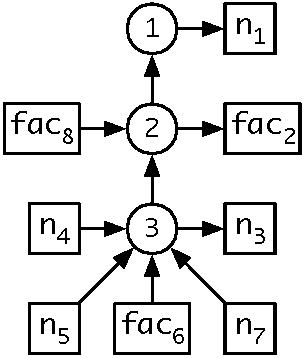
\includegraphics[scale=.5]{figures/examples/manual/02-scope}
\end{center}

\begin{mconstraints}{Declarations}
\EqCType{\dic{n}{1}}{\tau_{1}} &
\EqCType{\dic{n}{3}}{\intty{}} \\
\EqCTypeL{\dic{fac}{2}}{\arrty{\intty{}}{\intty{}}}
\end{mconstraints}
%
\begin{mconstraints}{Reference constraints}%
\EqCResolve{\ric{n}{4}}{\delta_{1}} &
\EqCType{\delta_{1}}{\intty{}}\\
\EqCResolve{\ric{n}{5}}{\delta_{2}} &
\EqCType{\delta_{2}}{\intty{}}\\
\EqCResolve{\ric{fac}{6}}{\delta_{3}} &
\EqCType{\delta_{3}}{\arrty{\tau_{6}}{\intty{}}}\\
\EqCResolve{\ric{n}{7}}{\delta_{4}} &
\EqCType{\delta_{4}}{\intty{}}\\
\EqCResolve{\ric{fac}{8}}{\delta_{5}} &
\EqCType{\delta_{5}}{\arrty{\tau_{8}}{\tau_{1}}}
\end{mconstraints}% 
}{%
\small
\begin{mconstraints}{Type constraints}
\EqCSubtype{\tau_{2}}{\arrty{\intty{}}{\intty{}}}\\
\EqCTeq{\tau_{2}}{\arrty{\intty{}}{\tau_{3}}}\\
\EqCTeq{\tau_{4}}{\intty{}}\\
\EqCTeq{\tau_{5}}{\intty{}}\\
\EqCTeq{\tau_{7}}{\intty{}}\\
\EqCSubtype{\tau_{7}}{\tau_{6}}\\
\EqCLub{\tau_{3}}{\tau_{4}}{\tau_{5}}\\
\EqCTeq{\tau_{9}}{\intty{}}\\
\EqCSubtype{\tau_{9}}{\tau_{8}}
\end{mconstraints}%
\begin{mconstraints}{Solution}
\RCSubst{\delta_{1}}{\dic{n}{3}} &
\RCSubst{\delta_{2}}{\dic{n}{3}}\\
\RCSubst{\delta_{3}}{\dic{fac}{2}} &
\RCSubst{\delta_{4}}{\dic{n}{3}}\\
\RCSubst{\delta_{5}}{\dic{fac}{2}} \\
\TCSubst{\tau_{1}}{\intty{}} &
\TCSubst{\tau_{3}}{\intty{}} \\
\TCSubst{\tau_{4}}{\intty{}} &
\TCSubst{\tau_{5}}{\intty{}} \\
\TCSubst{\tau_{6}}{\intty{}} &
\TCSubst{\tau_{7}}{\intty{}} \\
\TCSubst{\tau_{8}}{\intty{}} &
\TCSubst{\tau_{9}}{\intty{}} \\
\TCSubstL{\tau_{2}}{\arrty{\intty{}}{\intty{}}}
\end{mconstraints}%
}

\begin{boxedminipage}[t]{\hsize}
  \lstinputlisting[language=LMR,basicstyle=\lstfigurestyle, frame=none]{figures/examples/02-scope.lmr}
\end{boxedminipage}
\begin{boxedminipage}[t]{.545\hsize}
\usebox{\boxone}
\end{boxedminipage}
\hfill
\begin{boxedminipage}[t]{.445\hsize}
  \usebox{\boxtwo}%
  \vspace{\vdiff}
\end{boxedminipage}

\caption{Lexical scoping modeled in a scope graph and subtyping relations captured in constraints.}

  \figurelabel{lexical-scope}
\end{figure}

\Figure{lexical-scope} shows a larger LMR example that illustrates lexical scope
and subtype constraints.

Lexical scope is modeled using parent arrows between scopes in the scope graph.
In the example, scope 3, corresponding to the body of the \cod{fun}, is enclosed
in scope 2, corresponding to the \cod{letrec}, which is enclosed in scope 1, the
global scope of the program.
Resolution of a reference proceeds from the scope of the reference to parent
scopes until a matching declaration is found. 
Thus, reference $\ric{n}{5}$ resolves to declaration $\dic{n}{3}$, which shadows
$\dic{n}{1}$.

A function application such as \cod{fac$_6$(n$_7\;$ - 1)} requires that the type
of the actual parameter ($\tau_7$) is a subtype of the type of the
formal parameter ($\tau_6$).

\subsection{Imports}

\begin{figure}[t]
  \twoboxes{0.495\hsize}{0.495\hsize}{%
  \lstinputlisting[language=LMR,basicstyle=\lstfigurestyle, frame=none]{figures/examples/03-imports.lmr}
}{%
  \lstinputlisting[language=LMR,basicstyle=\lstfigurestyle, frame=none]{figures/examples/05-qualified.lmr}
}

\begin{boxedminipage}[t]{.495\hsize}
\usebox{\boxone}
\end{boxedminipage}
\hfill
\begin{boxedminipage}[t]{.495\hsize}
  \usebox{\boxtwo}%
  \vspace{\vdiff}
\end{boxedminipage}%
\twoboxes{0.495\hsize}{0.495\hsize}{%
\small
Scope graph

\begin{center}
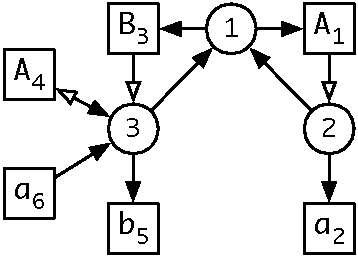
\includegraphics[scale=.5]{figures/examples/manual/03-imports}
\end{center}

\begin{mconstraints}{Declarations and constraints}
\EqCType{\dic{a}{2}}{\tau_{1}} & 
\EqCType{\dic{b}{5}}{\tau_{2}} \\
\EqCResolve{\ric{a}{6}}{\delta_{1}} &
\EqCType{\delta_{1}}{\intty{}}\\
\EqCTeq{\tau_{1}}{\intty{}} &
\EqCTeq{\tau_{2}}{\intty{}}
\end{mconstraints}%
\begin{mconstraints}{Solution}
\RCSubst{\delta_{1}}{\dic{a}{2}}\\
\TCSubst{\tau_{1}}{\intty{}} &
\TCSubst{\tau_{2}}{\intty{}}
\end{mconstraints}%
}{%
\small
Scope graph

\begin{center}
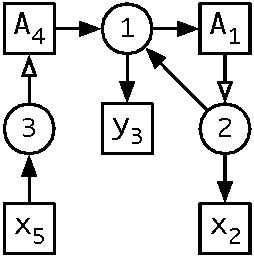
\includegraphics[scale=.5]{figures/examples/manual/05-qualified}
\end{center}

\begin{mconstraints}{Declarations and constraints}
\EqCType{\dic{x}{2}}{\tau_{1}} &
\EqCType{\dic{y}{3}}{\tau_{2}}
\\
\EqCResolve{\ric{x}{5}}{\delta_{1}} &
\EqCType{\delta_{1}}{\tau_{2}}
\\
\EqCTeq{\tau_{1}}{\intty{}}
\end{mconstraints}%
\begin{mconstraints}{Solution}
\RCSubst{\delta_{1}}{\dic{x}{2}}\\
\TCSubst{\tau_{1}}{\intty{}} &
\TCSubst{\tau_{2}}{\intty{}}
\end{mconstraints}%
}
\begin{boxedminipage}[t]{.495\hsize}
\usebox{\boxone}
\end{boxedminipage}
\hfill
\begin{boxedminipage}[t]{.495\hsize}
  \usebox{\boxtwo}%
  \vspace{\vdiff}
\end{boxedminipage}

\caption{Module imports and qualified names with example programs, scope graphs, and constraints.}

  \figurelabel{imports}
  \figurelabel{qualified-names}
\end{figure}

In addition to lexical scope, many programming languages provide features for
making declarations in scopes selectively available `at a distance'.
Examples of such constructs are modules with imports in ML and classes with
inheritance in Java.
To model such features, scope graphs provide \emph{associated scopes} and
\emph{imports}.

\paragraph{Associated Scope}

The LMR program in the left of \Figure{imports} consists of two \emph{modules} \cod{A$_1$}
and \cod{B$_3$} and an import from the former in the latter.
The declarations in these modules are contained in scopes 2 and 3, which are
child scopes of the root scope 1.
These scopes are \emph{associated} with the declaration of the name of the
module, which is represented in a scope graph diagram with an open arrow from
the declaration (e.g. $\dic{A}{1}$) to the scope (e.g. 2).

\paragraph{Imports}

The declarations in a scope are only visible to references in lexically enclosed
scopes, i.e. following parent edges to child scopes.
An \emph{import} makes the declarations in a scope visible in another, not
necessarily lexically related, scope.
An import is represented by (1) a regular reference of the
name in its enclosing scope, and (2) an import in that scope. The latter is
represented using an open arrow from a scope to a reference. For example,
\cod{import A$_4$} is represented by the reference $\ric{A}{4}$ in scope 3 and
an import arrow from scope 3 to $\ric{A}{4}$.

\paragraph{Resolving through Imports}

Name resolution in the presence of associated scopes and imports proceeds as
follows. 
If a scope $S_1$ contains an import $\ric{x}{i}$, which resolves to a
declaration $\dic{x}{j}$ with associated scope $S_2$, then all declarations in
$S_2$ are reachable in $S_1$.
Thus, in the example, reference $\ric{a}{6}$ resolves to declaration
$\dic{a}{2}$ since the import $\ric{A}{4}$ resolves to declaration 
$\dic{A}{1}$, and the associated scope 2 of $\dic{A}{1}$ contains declaration
$\dic{a}{2}$.
Note that the resolution calculus is parameterized with the
policy to disambiguate conflicting resolutions. Here we use the default policy
of \cite{NeronTVW-ESOP-2015} that prefers imported declarations over
declarations in parents.

\paragraph{Qualified Names}

Another common pattern for accessing the declarations in a scope is through
qualified names. Instead of importing \emph{all} declarations in a scope, a
single declaration is accessed. For example, in the right program from \Figure{qualified-names} the
expression \cod{A$_4$.x$_5$} refers to the declaration $\dic{x}{2}$ in module
\cod{A$_1$}. This pattern can be modeled using the scope graph ingredients that
we have seen so far.
The reference $\ric{x}{5}$ is defined as a reference of parentless scope 3. The
only declarations visible in scope 3 are through the import of $\ric{A}{4}$,
which is itself a reference in scope 1. Thus, since $\ric{A}{4}$ resolves to
$\dic{A}{1}$, the declarations in its associated scope 2 are visible in scope 3,
and therefore, $\ric{x}{5}$ resolves to $\dic{x}{2}$.



\subsection{Type-Dependent Name Resolution}

\begin{figure}[t]
  \twoboxes{0.495\hsize}{0.495\hsize}{%
  \lstinputlisting[language=LMR,basicstyle=\lstfigurestyle, frame=none]{figures/examples/06-fldaccess.lmr}
}{%
  \lstinputlisting[language=LMR,basicstyle=\lstfigurestyle, frame=none]{figures/examples/04-with-small.lmr}
}

\begin{boxedminipage}[t]{.495\hsize}
\usebox{\boxone}
\end{boxedminipage}
\hfill
\begin{boxedminipage}[t]{.495\hsize}
  \usebox{\boxtwo}%
  \vspace{\vdiff}
\end{boxedminipage}%
\twoboxes{0.495\hsize}{0.495\hsize}{%
\small
Scope graph

\begin{center}
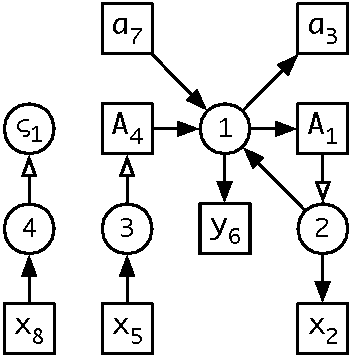
\includegraphics[scale=.5]{figures/examples/manual/06-fldaccess}
\end{center}

\begin{mconstraints}{Declarations}
\EqCType{\dic{x}{2}}{\intty{}} &
\EqCType{\dic{a}{3}}{\tau_{1}}\\
\EqCType{\dic{y}{6}}{\tau_{4}}
\end{mconstraints}
%
\begin{mconstraints}{Reference constraints}
\EqCResolve{\ric{A}{4}}{\delta_{1}}\\
\EqCResolve{\ric{x}{5}}{\delta_{2}} &
\EqCType{\delta_{2}}{\tau_{2}}\\
\EqCResolve{\ric{a}{7}}{\delta_{4}} &
\EqCType{\delta_{4}}{\recty{\delta_{3}}}\\
\EqCAssoc{\delta_{3}}{\varsigma_{1}}\\
\EqCResolve{\ric{x}{8}}{\delta_{5}} &
\EqCType{\delta_{5}}{\tau_{4}}
\end{mconstraints}% 
\begin{mconstraints}{Type constraints}
\EqCTeq{\tau_{1}}{\recty{\delta_{1}}} &
\EqCSubtype{\tau_{3}}{\tau_{2}}\\
\EqCTeq{\tau_{3}}{\intty{}}
\end{mconstraints}%
\begin{mconstraints}{Solution}
\RCSubst{\delta_{1}}{\dic{A}{1}} &
\RCSubst{\delta_{2}}{\dic{x}{2}}\\
\RCSubst{\delta_{3}}{\dic{A}{1}} &
\RCSubst{\delta_{4}}{\dic{a}{3}}\\
\RCSubst{\delta_{5}}{\dic{x}{2}} &
\RCSubst{\varsigma_{1}}{s_{2}}\\
\TCSubst{\tau_{1}}{\recty{\dic{A}{1}}} &
\TCSubst{\tau_{2}}{\intty{}}\\
\TCSubst{\tau_{3}}{\intty{}} &
\TCSubst{\tau_{4}}{\intty{}}
\end{mconstraints}%
}{%
\small
Scope graph

\begin{center}
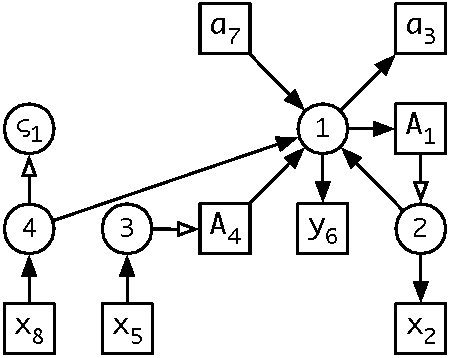
\includegraphics[scale=.5]{figures/examples/manual/04-with}
\end{center}

\begin{mconstraints}{Declarations}
\EqCType{\dic{x}{2}}{\intty{}} &
\EqCType{\dic{a}{3}}{\tau_{1}}\\
\EqCType{\dic{y}{6}}{\tau_{4}}
\end{mconstraints}
%
\begin{mconstraints}{Reference constraints}
\EqCResolve{\ric{A}{4}}{\delta_{1}} &
\EqCResolve{\ric{x}{5}}{\delta_{2}}\\
\EqCType{\delta_{2}}{\tau_{2}} &
\EqCResolve{\ric{a}{7}}{\delta_{4}}\\
\EqCType{\delta_{4}}{\recty{\delta_{3}}} &
\EqCAssoc{\delta_{3}}{\varsigma_{1}}\\
\EqCResolve{\ric{x}{8}}{\delta_{5}} &
\EqCType{\delta_{5}}{\intty{}}
\end{mconstraints}% 
\begin{mconstraints}{Type constraints}
\EqCTeq{\tau_{1}}{\recty{\delta_{1}}} &
\EqCSubtype{\tau_{3}}{\tau_{2}} \\
\EqCTeq{\tau_{3}}{\intty{}} &
\EqCTeq{\tau_{4}}{\intty{}}
\end{mconstraints}%
\begin{mconstraints}{Solution}
\RCSubst{\delta_{1}}{\dic{A}{1}}&
\RCSubst{\delta_{2}}{\dic{x}{2}}\\
\RCSubst{\delta_{3}}{\dic{A}{1}}&
\RCSubst{\delta_{4}}{\dic{a}{3}}\\
\RCSubst{\delta_{5}}{\dic{x}{2}}&
\RCSubst{\varsigma_{1}}{s_{2}}\\
\TCSubst{\tau_{1}}{\recty{\dic{A}{1}}}&
\TCSubst{\tau_{2}}{\intty{}}\\
\TCSubst{\tau_{3}}{\intty{}}&
\TCSubst{\tau_{4}}{\intty{}}
\end{mconstraints}%
}
\begin{boxedminipage}[t]{.495\hsize}
\usebox{\boxone}
\end{boxedminipage}
\hfill
\begin{boxedminipage}[t]{.495\hsize}
  \usebox{\boxtwo}%
  \vspace{\vdiff}
\end{boxedminipage}

\caption{Field Access and \cod{with} expression modeled by virtual scopes, reference, association, and type constraints.}

  \figurelabel{field-access}
  \figurelabel{with}
\end{figure}

To summarize, scope graphs provide a language-independent model for formalizing
the binding rules in programming languages. Neron et al.
\cite{NeronTVW-ESOP-2015} show that the approach covers a wide range of name
binding idioms.
In this section we have shown that scope graphs can be complemented with type
constraints to express the static typing requirements on programs (to be
formalized later in this paper).
These constraints use name resolution constraints to express the dependence of
type resolution on name resolution.

However, for some language constructs the resolution of a name to its
declaration depends on the type of another expression.
For example, in field access expression \cod{e.f}, in order to resolve the field
\cod{f}, one first needs to find the type of the expression \cod{e} and then to
look for \cod{f} in the scope associated with the type.
This scheme induces a dependency, not only of the name resolution but also of
the scope graph construction (one does not know in which scope the reference
\cod{f} lies) on the type resolution.
We model such \emph{type-dependent name resolution} by means of constraints over
the edges in the scope graph.

\paragraph{Field Access}

Both examples in \Figure{field-access} illustrate the approach. In the left example, we
are particularly interested in the field access in the definition of $\dic{y}{6}$.
The reference $\ric{x}{8}$ is a field access in the record value of
$\ric{a}{7}$.
Thus, $\ric{x}{8}$ should be resolved in the associated scope of the type of the
receiver expression $\ric{a}{7}$.
This is similar to the resolution of a qualified name, which we modeled by
resolving the qualified name in a parentless scope into which we imported the
module.
Thus, we create a parentless scope (4) and add $\ric{x}{8}$ as reference in that
scope.
However, in this case we do not know (the name of) the record type that should
be imported into the parentless scope.
Therefore, we proceed as follows.
We create a new scope identified by a \emph{scope variable} $\varsigma_1$  that
acts as a placeholder for the scope that we want to import into the parentless
scope 4.
We add a \emph{direct import edge} (open arrow) from scope 4 to scope
$\varsigma_1$.
Then, we resolve $\ri{a}{7}$ using $\CResolve{\ri{a}{7}}{\delta_{4}}$ and obtain
the type of its definition through $\CType{\delta_{4}}{\recty{\delta_{3}}}$,
which should be a record type identifying the record definition $\delta_3$.
Using a constraint $\CAssoc{\delta_{3}}{\varsigma_{1}}$ over the scope graph, we
obtain the associated scope of the record definition.
Solving these constraints will lead to a solution for $\varsigma_{1}$ --- in
this case the associated scope of $\dic{A}{1}$, scope 2 --- such that the
appropriate scope can be imported into scope 4.
After that $\ri{x}{8}$ can be resolved as usual to its definition
$\CResolve{\ri{x}{8}}{\delta_{5}}$, which leads to its type
$\CType{\delta_{5}}{\tau_{4}}$.

Note that scope 3 and related edges and constraints model the resolution of the
field initializer in the definition of $\dic{a}{3}$, which is similar to the
pattern for qualified names, but applies to a list of initializer expressions.

\paragraph{With}

As final example, we discuss an expression form inspired by the \cod{with} statement
in the Pascal language. In the expression \cod{with e do e'}, the fields of the record
value of \cod{e} are added to the lexical environment of \cod{e'}. That is, a
variable reference \cod{x} in \cod{e'} will be interpreted as a field of the
record value when the record has indeed a field with name \cod{x}; otherwise the
variable is considered as a regular reference in the enclosing lexical context.
Static resolution again requires resolving variables in \cod{e'} in the
associated scope of the record type of \cod{e}, but this time defaulting to the enclosing
lexical scope.

\Figure{with} shows on its right how this is modeled for the expression \cod{with a$_7\;$  do
x$_8\;$ + 1} using a scope (4) that directly imports a placeholder scope
($\varsigma_{1}$) as the lexical context for the references in the body of the
\cod{with}. The scope variable is resolved through the constraints
$\CResolve{\ri{a}{7}}{\delta_{4}}$, $\CType{\delta_{4}}{\recty{\delta_{3}}}$,
and $\CAssoc{\delta_{3}}{\varsigma_{1}}$ to the associated scope of the type of
$\ric{a}{7}$.
Unlike in the case of field access the scope for the body of the \cod{with}
\emph{does} have a parent scope (1), so that references that are not to fields
of the record are resolved in the lexical context.

\subsection{Roadmap}

The rest of this paper formalizes the approach to type-dependent name resolution
sketched in this section.
\Section{extscopegraph} reviews the resolution calculus of Neron et al.
\cite{NeronTVW-ESOP-2015} and extends it with direct imports between scopes. 
\Section{constraintlang} defines the syntax and semantics of a constraint
language that can be used by language front-ends to express the name binding and
type rules of a language. 
In \Section{collection} we give a complete account of
extraction of constraints for all LMR constructs. 
\Section{resolution-algorithm} describes a resolution algorithm that finds
solutions for resolution problems.

\endinput


\subsection{Name and Type Resolution}

explain scope graphs concepts: declarations, references, scopes, and imports

we show how type resolution is complementary to name resolution and can be
described using equality and subtype constraints on types and name resolution
constraints

we illustrate the interaction between name resolution and type resolution using
nominal record types, and the field access and with constructs

we show how the interaction is modeled using the extension of scope graphs with
direct (nameless) imports

separation of name resolution and typing

type constraints
    


we have language-independent representation for scope graphs, but we did not
yet have a good way of defining the extraction; the imperative operations in
ESOP are ugly; scope graph constraints (assumptions) provide the basic building
blocks for a high-level extraction DSL


the resolution calculus does not say anything about types and we need to
combine name resolution with type analysis to define type systems; how do we
express type analysis in a scope graph world (even without the interaction)

(while mostly independent, names and types do interact; how to model that?

types depend on names; lookup type of variable

but names also depend on types; field acces, with, \ldots


Name resolution as presented in \cite{NeronTVW-ESOP-2015} relies on a two stage
approach. First a language-dependent procedure extracts a scope graph from the
program AST. Then a language-independent procedure resolves the references in
the program to their declarations by finding paths in the scope graph.

With explicit typing, typing rules can simply use the resolution relation to
recover the type of a variable reference by using the type that is declared at
the variable declaration site.

This makes the type resolution depend on name resolution. 

However, for some language constructs the resolution of a name to its
declaration depends on the type of another expression.

For example, in field access, {\sf a.x}, in order to resolve {\sf x}, one first
needs to find the type of {\sf a} and then to look for {\sf x} in that type
definition.

This scheme induces a dependency, not only of the name
resolution but also of the scope graph construction (one does not know in which
scope the reference {\sf x} lies) on the type resolution.

\subsection{Constraints}

\TODO{The constraint language provides a linguistic interface between the
language-dependendent extraction and the language-independent scope graph
representation and resolution algorithm. }

The constraint approach allows us to resolve this mutual dependency by
generating constrained not only related to the type resolution but also to the
scope graph construction and the name resolution.

The resolution of a program first involves a collection of the constraints
relative to this program using an AST traversal. Constraints generated by this
traversal are not only related to typing but also to the scope graph
construction and the name resolution. Therefore these constraints relate not
only types but also scopes, references, declarations and positions of the
program AST. All these elements can also be represented using variables of the
corresponding sort in the constraint language (that we usually denote with greek
letters). 
One well-known mechanism for type resolution,
which meets our formalism criteria above, is based on 
extracting {\it constraints} on types and type variables
from the AST and then using {\it unification} to solve the constraints
and instantiate the variables.
This technique goes back at least to Milner's seminal paper on polymorphism~\cite{Milner78:0},
and has since been extended to cover many additional language features,
notably subtyping; Pottier and Remy~(Chapter 10 of \cite{Pierce05advancedtopics}) give a detailed exposition,
and show how an efficient resolution algorithm can be expressed using rewrite rules. 
The constraint approach is most commonly used for 
type inference, but even for the simpler problem of type checking, 
passing to constraints is a useful way to separate the language-dependent
part of the task (generating the constraints) from the language-independent part
(solving the constaints).

Figure~\ref{fig:simple-constraints} illustrates how a constraint-based approach
to type checking might work on top of name resolution for a small fragment of a
simple monomorphically-typed language. At the top of the figure, we show the set
of constraints, obtained by walking over the program AST; we defer discussion of
the details of constraint generation to a later section.
\begin{figure}[tb]
\begin{boxedminipage}{\hsize}
\center{
Constraints (where overall program type is $\tau_0$)}
\[
\begin{array}{rcl}
\tau_0 & = & \mbox{\tt Int} \rightarrow \tau_1  \\
\tau_1 & = & \mbox{\tt Bool} \rightarrow \tau_2  \\
\ri{y}{4} & \resolve & \di{y}{\iota_1} \\
\typeat{\iota_1} & = & \mbox{\tt Bool}\\
\ri{y}{5} & \resolve & \di{y}{\iota_2} \\
\typeat{\iota_2} & = & \mbox{\tt Bool} \\
\ri{x}{6} & \resolve & \di{x}{\iota_3} \\
\typeat{\iota_3} & = & \tau_2\\
\end{array}
\]
\end{boxedminipage}
\\
\begin{boxedminipage}{\hsize}
\center{Solution to constraints}
\\
$\iota_1 = 2$, $\iota_2 = 2$, $\iota_3 = 3$,
$\tau_2 = \mbox{\tt Bool}$,\\
$\tau_1 = \mbox{\tt Bool} \rightarrow \mbox{\tt Bool}$,
$\tau_0 = \mbox{\tt Int} \rightarrow \mbox{\tt Bool} \rightarrow \mbox{\tt Bool}$
\end{boxedminipage}
\caption{Constraints for Simple Program}
\label{fig:simple-constraints}
\end{figure}
There are two forms of constraints: conventional type equalities,
and name resolution constraints.  The latter replace the implicit
name resolution via manipulation of a typing context that would 
be used in a more conventional presentation.
Note that constraints can
mention {\em position variables} $\iota$ as well as ordinary type variables
$\tau$.  At the bottom of the figure, we show a solution to the constraint set, 
written as a substiution on type and position variables. The solution is
obtained  by plugging in the facts about $\resolve$ and $\typeat{}$ derived 
from the scope graph, and then performing unification; again, we defer details
to a later section.



\subsection{Scope}

\subsection{Imports}

\subsection{Qualified Names}

This simple two stage approach---name resolution using the
scope graph followed by separate type resolution---will work for
many language constructs. But the full story is more complicated,
because sometimes name resolution also depends on type resolution.
Consider the program fragments in Figure~\ref{fig:records-program}, written
in a language having nominal records and using standard dot notation 
for record field access. 

In a scope graph setting, we can create one scope that contains
the field declaration of record type \cod{A$_1$}, and another that
contains those of \cod{B$_3$}, and associate each scope with the
corresponding type name.
Now, in order to resolve the type of \cod{y$_7$.x$_8$} we must first 
resolve the field name \cod{x$_8$} to the appropriate
declaration field (\cod{x$_2$} or \cod{x$_6$}). 
But this name resolution depends on the {\it type} of \cod{y$_7$},
so we must resolve that type first.  
In general, we may need arbitrarily deep recursion between
the two kinds of resolution. For example, to handle the nested 
record dereference on the last line, we must first resolve the name
of \cod{y$_9$}, then its type, then the name and type of \cod{a$_{10}$}, 
and finally the name and type of \cod{x$_{11}$}. 

To solve this challenge, we 
reformulate the task of generating a scope graph from a given program
as one of finding a minimal solution to a set of {\it scope constraints}
obtained by an AST traversal.
Scope constraints are analogous to typing constraints, 
but are resolved using a different (and simpler) algorithm.
We then introduce a class of {\it scope variables} and modify
the resolution calculus to characterize resolution in potentially {\it incomplete} 
scope graphs (i.e., graphs characterized by constraints involving unresolved 
scope variables).
We can then interleave (partial) scope graph resolution and type unification 
until a complete instantiation of all variables (types, positions, and
scopes) is obtained.  This approach permits us to resolve all the names
and types for the record examples of Figure~\ref{fig:records-program} 
and for a broad range of other language constructs. 



\subsection{}


    
    example scope graphs + types for interesting examples
    
    can we draw those? or do we use constraints? but those are not so easy to read
    
    consider example programs + scope graphs + type assignments, 
    
i.e. the result of resolution

discuss what the solutions for type-dependent problems look like


the difference between \lstinline+x : Int+ and \lstinline+record A { ... }+ is
that the first is an identifier with a type, and the second is an identifier that defines a type








%\newsavebox\boxfix
\newsavebox\boxfun
\newsavebox\boxifz
\newsavebox\boxone
\newsavebox\boxexp
\newsavebox\boxapp
\newsavebox\boxarg
\newsavebox\boxint
\savebox\boxfix{\codefig{fix ...}}
\savebox\boxfun{\codefig{fun ...}}
\savebox\boxifz{\codefig{ifz ...}}
\savebox\boxone{\codefig{1}}
\savebox\boxexp{\codefig{n$_5$*f$_6$(n$_7$-1)}}
\savebox\boxapp{\codefig{f$_6$(n$_7$-1)}}
\savebox\boxarg{\codefig{n$_7$-1}}
\savebox\boxint{\codefig{Int}}
\begin{figure}
\begin{boxedminipage}{0.495\hsize}
\begin{lstlisting}[language=LMR,basicstyle=\lstfigurestyle,breaklines=true,frame=none]
def f$_1$:Int->Int =
  fix f$_2$:Int->Int {
    fun n$_3$:Int {
      ifz n$_4$ then 1
      else n$_5$*f$_6$(n$_7$-1)
    }
  }
def n$_8$:Int = f$_9$ 5
\end{lstlisting}
\end{boxedminipage}\hfill
\begin{boxedminipage}{0.495\hsize}
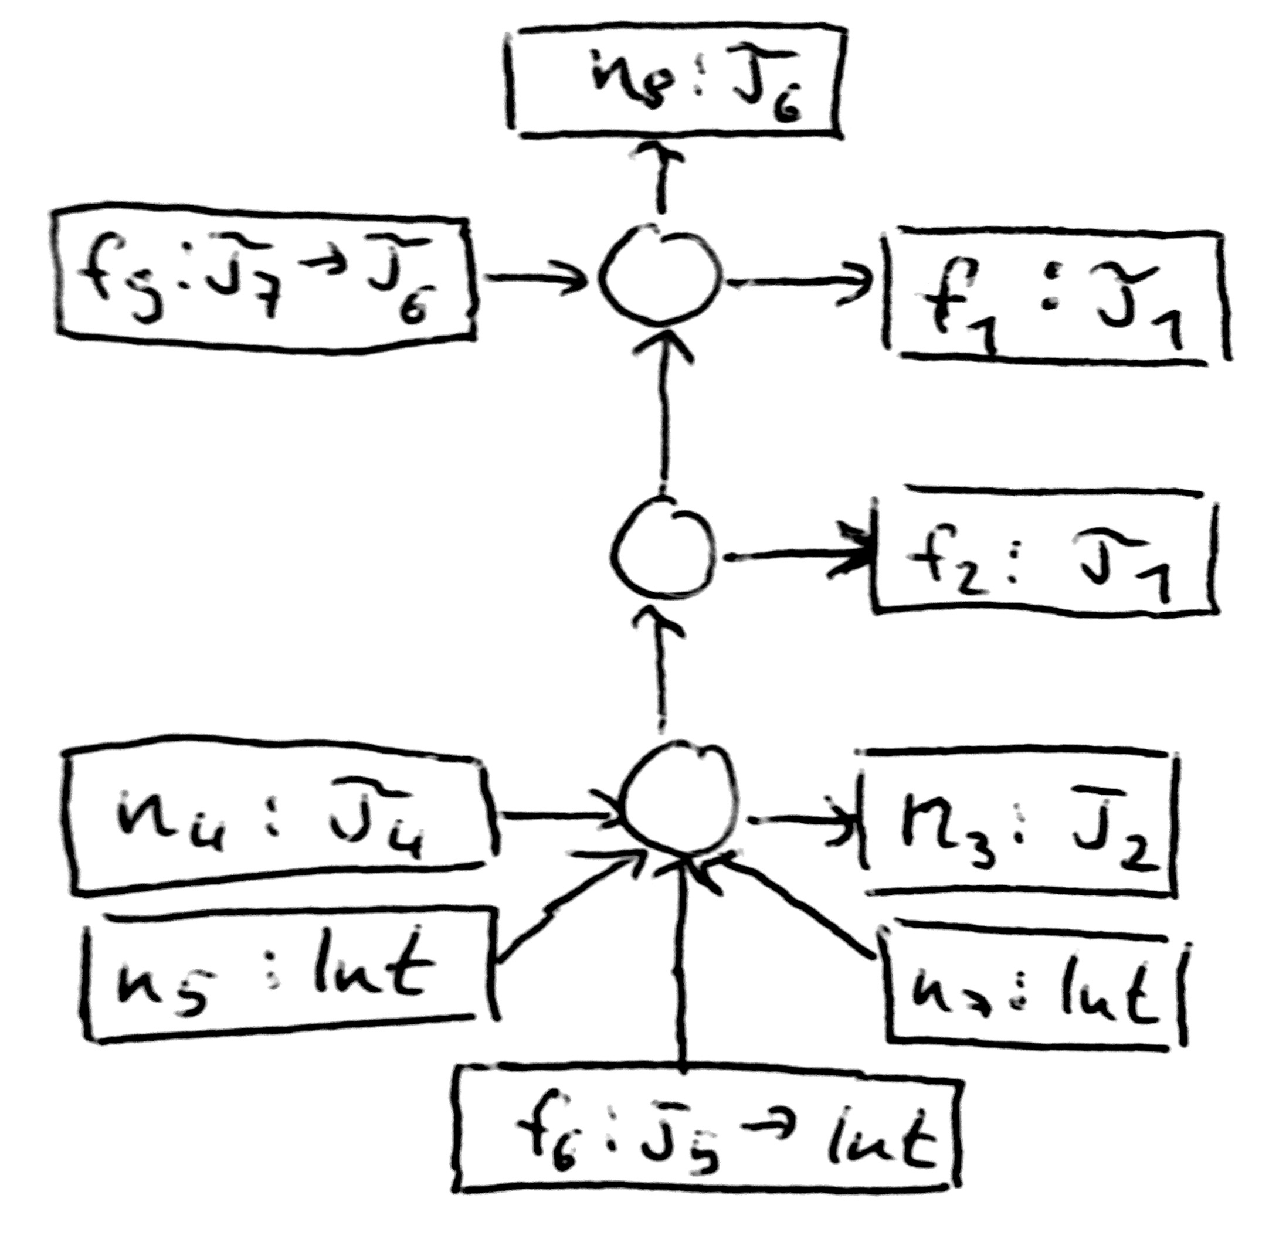
\includegraphics[width=\hsize]{figures/infgraph.pdf}
\end{boxedminipage}
\begin{boxedminipage}{0.495\hsize}
\small
\center{type constraints}
\[
\begin{array}{l}
\ceq{\vty{2} \rightarrow \vty{3}}{\usebox{\boxint} \rightarrow \usebox{\boxint}}\\
\ceq{\vty{4}}{\usebox{\boxint}}\\
\ceq{\usebox{\boxint}}{\vty{3}}\\
\ceq{\usebox{\boxint}}{\vty{5}}\\
\end{array}
\]
\end{boxedminipage}\hfill
\begin{boxedminipage}{0.495\hsize}
\small
\center{solutions to constraints}
\[
\begin{array}{l}
\ceq{\vty{2}}{\usebox{\boxint}}\\
\ceq{\vty{3}}{\usebox{\boxint}}\\
\ceq{\vty{4}}{\usebox{\boxint}}\\
\ceq{\vty{5}}{\usebox{\boxint}}
\end{array}
\]
\end{boxedminipage}

\label{fig:checking}
\caption{Type checking.}
\end{figure}

%\begin{figure}
\begin{boxedminipage}{0.495\hsize}
\begin{lstlisting}[language=LMR,basicstyle=\lstfigurestyle,breaklines=true,frame=none]
def f$_1$:Int->Int =
  fix f$_2$:Int->Int {
    fun n$_3$:Int {
      ifz n$_4$ then 1
      else n$_5$*f$_6$(n$_7$-1)
    }
  }
def n$_8$:Int = f$_9$ 5
\end{lstlisting}
\end{boxedminipage}\hfill
\begin{boxedminipage}{0.495\hsize}
\begin{lstlisting}[language=LMR,basicstyle=\lstfigurestyle,breaklines=true,frame=none]
def f$_1$ =
  fix f$_2$ {
    fun n$_3$ {
      ifz n$_4$ then 1
      else n$_5$*f$_6$(n$_7$-1)
    }
  }
def n$_8$ = f$_9$ 5
\end{lstlisting}
\end{boxedminipage}

\begin{boxedminipage}{\hsize}
\small
\center{scope graph}
\[
\begin{array}{llll}
\froot{1}\\
\fdec{f}{1}{1} & \fpar{2}{1} \\
\fdec{f}{2}{2} & \fpar{3}{2} \\
\fdec{n}{3}{3} \\
\fref{n}{4}{3} & \fref{n}{5}{3} & \fref{f}{6}{3} & \fref{n}{7}{3} \\
\fdec{n}{8}{3} & \fref{f}{9}{1}
\end{array}
\]
\end{boxedminipage}
\begin{boxedminipage}{\hsize}
\small
\center{resolution constraints}
\[
\begin{array}{llll}
\cresolves{n}{4}{1} & \cresolves{n}{5}{2} & 
\cresolves{f}{6}{3} & \cresolves{n}{7}{4} \\
\cresolves{f}{9}{5}
\end{array}
\]
\end{boxedminipage}
\begin{boxedminipage}{0.495\hsize}
\small
\center{type assumptions}
\[
\begin{array}{llll}
\fdecty{f}{1}{\usebox{\boxint} \rightarrow \usebox{\boxint}} \\
\cty{\usebox{\boxfix}}{\usebox{\boxint} \rightarrow \usebox{\boxint}}\\
%
\fdecty{f}{2}{\usebox{\boxint} \rightarrow \usebox{\boxint}} \\
\cty{\usebox{\boxfun}}{\usebox{\boxint} \rightarrow \usebox{\boxint}}\\
%
\fdecty{n}{3}{\usebox{\boxint}} \\
\cty{\usebox{\boxifz}}{\vty{3}}\\
%
\cty{\ri{n}{4}}{\vty{4}}\\
\cty{\usebox{\boxone}}{\vty{3}}\\
\cty{\usebox{\boxexp}}{\vty{3}}\\
%
\cty{\ri{n}{5}}{\usebox{\boxint}}\\
\cty{\usebox{\boxapp}}{\usebox{\boxint}}\\
%
\cty{\ri{f}{6}}{\vty{5}\rightarrow \usebox{\boxint}}\\
\cty{\usebox{\boxarg}}{\vty{5}}\\
%
\cty{\ri{n}{7}}{\usebox{\boxint}}\\
\end{array}
\]
\center{type constraints}
\[
\begin{array}{llll}
\ceq{\vty{2} \rightarrow \vty{3}}{\usebox{\boxint} \rightarrow \usebox{\boxint}}\\
%
\cty{\vdec{1}}{\vty{4}} \\
\ceq{\vty{4}}{\usebox{\boxint}}\\
%
\ceq{\usebox{\boxint}}{\vty{3}}\\
%
%\ceq{\usebox{\boxint}}{\vty{3}}\\
%
\cty{\vdec{2}}{\usebox{\boxint}}\\
%
\cty{\vdec{3}}{\vty{5}\rightarrow \usebox{\boxint}}\\
%
\ceq{\usebox{\boxint}}{\vty{5}}\\
\cty{\vdec{4}}{\usebox{\boxint}}\\
\cty{\usebox{\boxone}}{\usebox{\boxint}}\\
\end{array}
\]
\end{boxedminipage}\hfill
\begin{boxedminipage}{0.495\hsize}
\small
\center{type assumptions}
\[
\begin{array}{llll}
\fdecty{f}{1}{\vty{1}} \\
\cty{\usebox{\boxfix}}{\vty{1}}\\
%
\fdecty{f}{2}{\vty{1}} \\
\cty{\usebox{\boxfun}}{\vty{1}}\\
%
\fdecty{n}{3}{\vty{2}} \\
\cty{\usebox{\boxifz}}{\vty{3}}\\
%
\cty{\ri{n}{4}}{\vty{4}}\\
\cty{\usebox{\boxone}}{\vty{3}}\\
\cty{\usebox{\boxexp}}{\vty{3}}\\
%
\cty{\ri{n}{5}}{\usebox{\boxint}}\\
\cty{\usebox{\boxapp}}{\usebox{\boxint}}\\
%
\cty{\ri{f}{6}}{\vty{5}\rightarrow \usebox{\boxint}}\\
\cty{\usebox{\boxarg}}{\vty{5}}\\
%
\cty{\ri{n}{7}}{\usebox{\boxint}}\\
\end{array}
\]
\center{type constraints}
\[
\begin{array}{llll}
\ceq{\vty{2} \rightarrow \vty{3}}{\vty{1}}\\
%
\cty{\vdec{1}}{\vty{4}} \\
\ceq{\vty{4}}{\usebox{\boxint}}\\
%
\ceq{\usebox{\boxint}}{\vty{3}}\\
%
%\ceq{\usebox{\boxint}}{\vty{3}}\\
%
\cty{\vdec{2}}{\usebox{\boxint}}\\
%
\cty{\vdec{3}}{\vty{5}\rightarrow \usebox{\boxint}}\\
\ceq{\usebox{\boxint}}{\vty{5}}\\
\cty{\vdec{4}}{\usebox{\boxint}}\\
\cty{\usebox{\boxone}}{\usebox{\boxint}}\\
\end{array}
\]
\end{boxedminipage}
\begin{boxedminipage}{\hsize}
\small
\center{solution to constraints}
\[
\begin{array}{lllll}
\sdec{1}{n}{3} & \sdec{2}{n}{3} & \sdec{3}{f}{2} & \sdec{4}{n}{3}
& \sdec{5}{f}{1}
\end{array}
\]
\end{boxedminipage}
\label{fig:lexical-scope}
\caption{Lexical scoping modeled by edges between scopes.}
\end{figure}


%\begin{figure}
\begin{boxedminipage}{0.495\hsize}
\begin{lstlisting}[language=LMR,basicstyle=\lstfigurestyle,breaklines=true,frame=none]
def f$_1$ =
  fix f$_2$ {
    fun n$_3$ {
      ifz n$_4$ then 1
      else n$_5$*f$_6$(n$_7$-1)
    }
  }
def n$_8$ = f$_9$ 5
\end{lstlisting}
\end{boxedminipage}\hfill
\begin{boxedminipage}{0.495\hsize}
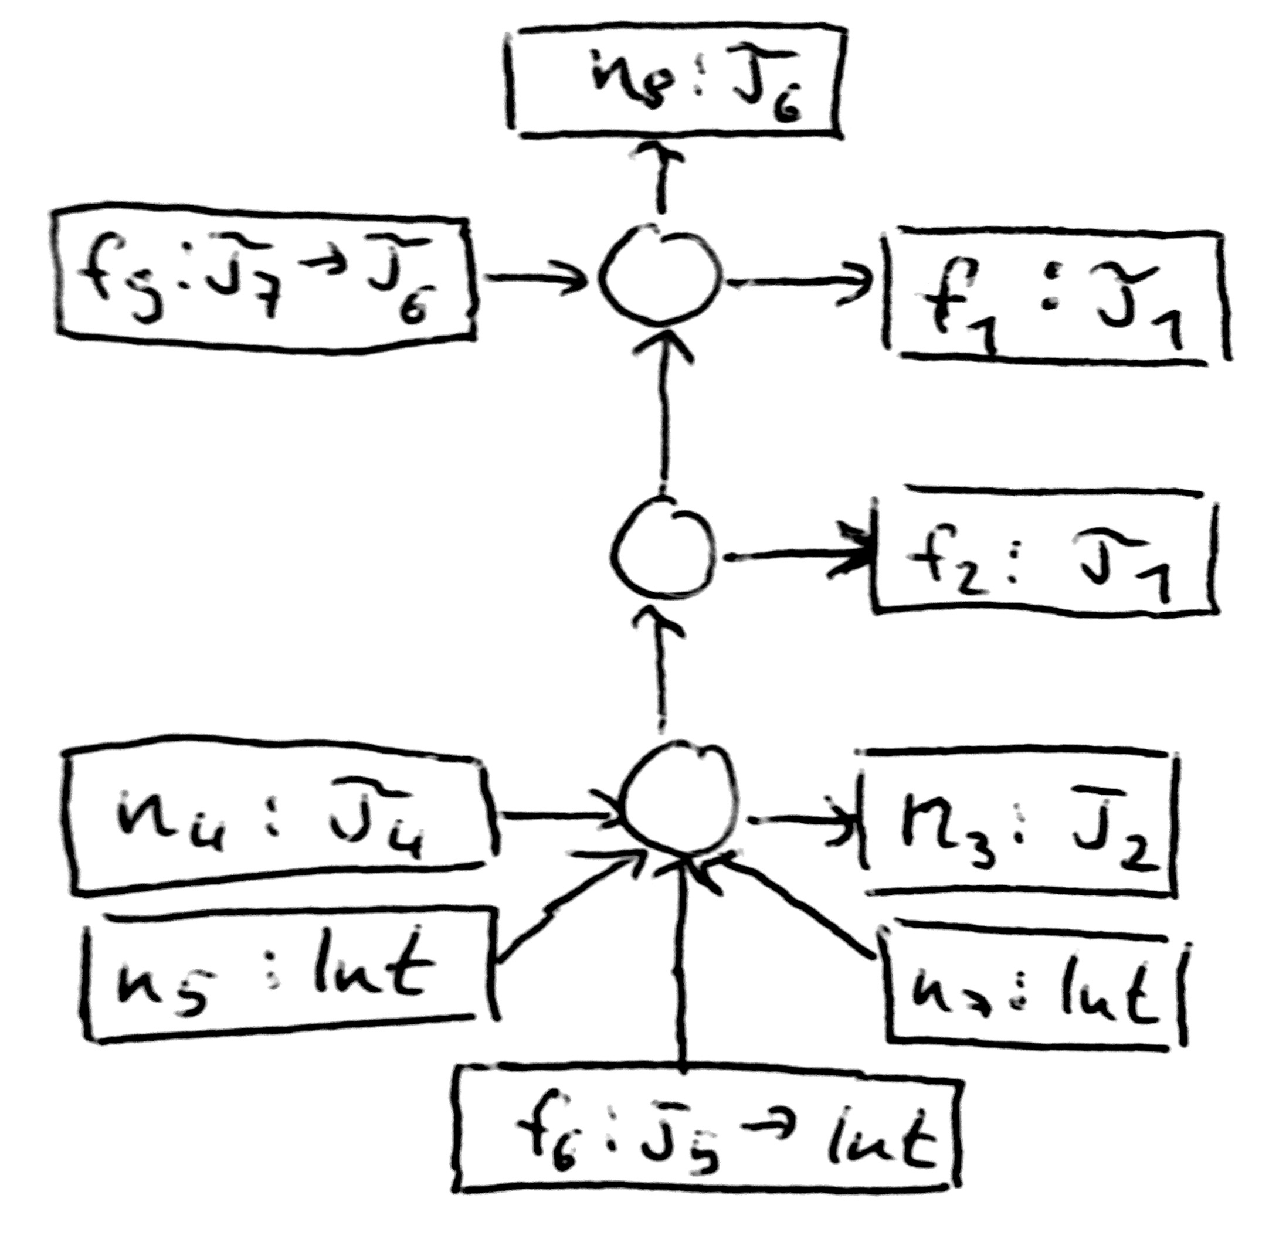
\includegraphics[width=\hsize]{figures/infgraph.pdf}
\end{boxedminipage}
\begin{boxedminipage}{0.495\hsize}
\small
\center{type constraints}
\[
\begin{array}{l}
\ceq{\vty{2} \rightarrow \vty{3}}{\vty{1}}\\
\ceq{\vty{4}}{\usebox{\boxint}}\\
\ceq{\usebox{\boxint}}{\vty{3}}\\
\ceq{\usebox{\boxint}}{\vty{5}}\\
\end{array}
\]
\vfill
\end{boxedminipage}\hfill
\begin{boxedminipage}{0.495\hsize}
\small
\center{solutions to constraints}
\[
\begin{array}{l}
\ceq{\vty{1}}{\usebox{\boxint} \rightarrow \usebox{\boxint}}\\
\ceq{\vty{2}}{\usebox{\boxint}}\\
\ceq{\vty{3}}{\usebox{\boxint}}\\
\ceq{\vty{4}}{\usebox{\boxint}}\\
\ceq{\vty{5}}{\usebox{\boxint}}
\end{array}
\]
\end{boxedminipage}

\label{fig:inference}
\caption{Type inference.}
\end{figure}



% \begin{figure}
% \begin{lstlisting}[language=LMR,basicstyle=\lstfigurestyle,breaklines=true]
% fun y$_1$:Int { 
%   fun y$_2$:Bool { 
%     let x$_3$:Bool = if y$_4$ then True else y$_5$ 
%     in x$_6$
%   }
% }
% \end{lstlisting}
% \label{fig:simple-prog}
% \caption{A simple program}
% \end{figure}

% \subsection{Scope Graphs}
% 
% 
% \subsection{Resolution}
% 
% \subsection{Type Checking}
% 
% 
% \subsection{Type Inference}
% 
% 
% 
% \subsection{Nominal Types}
% 
% \subsection{Type-Dependent Resolution}
% 
% \subsection{Nominal Subtyping}
